% Options for packages loaded elsewhere
\PassOptionsToPackage{unicode}{hyperref}
\PassOptionsToPackage{hyphens}{url}
%
\documentclass[
]{article}
\usepackage{amsmath,amssymb}
\usepackage{lmodern}
\usepackage{ifxetex,ifluatex}
\ifnum 0\ifxetex 1\fi\ifluatex 1\fi=0 % if pdftex
  \usepackage[T1]{fontenc}
  \usepackage[utf8]{inputenc}
  \usepackage{textcomp} % provide euro and other symbols
\else % if luatex or xetex
  \usepackage{unicode-math}
  \defaultfontfeatures{Scale=MatchLowercase}
  \defaultfontfeatures[\rmfamily]{Ligatures=TeX,Scale=1}
\fi
% Use upquote if available, for straight quotes in verbatim environments
\IfFileExists{upquote.sty}{\usepackage{upquote}}{}
\IfFileExists{microtype.sty}{% use microtype if available
  \usepackage[]{microtype}
  \UseMicrotypeSet[protrusion]{basicmath} % disable protrusion for tt fonts
}{}
\makeatletter
\@ifundefined{KOMAClassName}{% if non-KOMA class
  \IfFileExists{parskip.sty}{%
    \usepackage{parskip}
  }{% else
    \setlength{\parindent}{0pt}
    \setlength{\parskip}{6pt plus 2pt minus 1pt}}
}{% if KOMA class
  \KOMAoptions{parskip=half}}
\makeatother
\usepackage{xcolor}
\IfFileExists{xurl.sty}{\usepackage{xurl}}{} % add URL line breaks if available
\IfFileExists{bookmark.sty}{\usepackage{bookmark}}{\usepackage{hyperref}}
\hypersetup{
  pdftitle={Factors influencing Scots' satisfaction with public transport},
  pdfauthor={Group 28: Aishwin Tikku, Mengran Li, Steven Kwok, Shaoquan Li, Shuning Li},
  hidelinks,
  pdfcreator={LaTeX via pandoc}}
\urlstyle{same} % disable monospaced font for URLs
\usepackage[margin=1in]{geometry}
\usepackage{color}
\usepackage{fancyvrb}
\newcommand{\VerbBar}{|}
\newcommand{\VERB}{\Verb[commandchars=\\\{\}]}
\DefineVerbatimEnvironment{Highlighting}{Verbatim}{commandchars=\\\{\}}
% Add ',fontsize=\small' for more characters per line
\usepackage{framed}
\definecolor{shadecolor}{RGB}{248,248,248}
\newenvironment{Shaded}{\begin{snugshade}}{\end{snugshade}}
\newcommand{\AlertTok}[1]{\textcolor[rgb]{0.94,0.16,0.16}{#1}}
\newcommand{\AnnotationTok}[1]{\textcolor[rgb]{0.56,0.35,0.01}{\textbf{\textit{#1}}}}
\newcommand{\AttributeTok}[1]{\textcolor[rgb]{0.77,0.63,0.00}{#1}}
\newcommand{\BaseNTok}[1]{\textcolor[rgb]{0.00,0.00,0.81}{#1}}
\newcommand{\BuiltInTok}[1]{#1}
\newcommand{\CharTok}[1]{\textcolor[rgb]{0.31,0.60,0.02}{#1}}
\newcommand{\CommentTok}[1]{\textcolor[rgb]{0.56,0.35,0.01}{\textit{#1}}}
\newcommand{\CommentVarTok}[1]{\textcolor[rgb]{0.56,0.35,0.01}{\textbf{\textit{#1}}}}
\newcommand{\ConstantTok}[1]{\textcolor[rgb]{0.00,0.00,0.00}{#1}}
\newcommand{\ControlFlowTok}[1]{\textcolor[rgb]{0.13,0.29,0.53}{\textbf{#1}}}
\newcommand{\DataTypeTok}[1]{\textcolor[rgb]{0.13,0.29,0.53}{#1}}
\newcommand{\DecValTok}[1]{\textcolor[rgb]{0.00,0.00,0.81}{#1}}
\newcommand{\DocumentationTok}[1]{\textcolor[rgb]{0.56,0.35,0.01}{\textbf{\textit{#1}}}}
\newcommand{\ErrorTok}[1]{\textcolor[rgb]{0.64,0.00,0.00}{\textbf{#1}}}
\newcommand{\ExtensionTok}[1]{#1}
\newcommand{\FloatTok}[1]{\textcolor[rgb]{0.00,0.00,0.81}{#1}}
\newcommand{\FunctionTok}[1]{\textcolor[rgb]{0.00,0.00,0.00}{#1}}
\newcommand{\ImportTok}[1]{#1}
\newcommand{\InformationTok}[1]{\textcolor[rgb]{0.56,0.35,0.01}{\textbf{\textit{#1}}}}
\newcommand{\KeywordTok}[1]{\textcolor[rgb]{0.13,0.29,0.53}{\textbf{#1}}}
\newcommand{\NormalTok}[1]{#1}
\newcommand{\OperatorTok}[1]{\textcolor[rgb]{0.81,0.36,0.00}{\textbf{#1}}}
\newcommand{\OtherTok}[1]{\textcolor[rgb]{0.56,0.35,0.01}{#1}}
\newcommand{\PreprocessorTok}[1]{\textcolor[rgb]{0.56,0.35,0.01}{\textit{#1}}}
\newcommand{\RegionMarkerTok}[1]{#1}
\newcommand{\SpecialCharTok}[1]{\textcolor[rgb]{0.00,0.00,0.00}{#1}}
\newcommand{\SpecialStringTok}[1]{\textcolor[rgb]{0.31,0.60,0.02}{#1}}
\newcommand{\StringTok}[1]{\textcolor[rgb]{0.31,0.60,0.02}{#1}}
\newcommand{\VariableTok}[1]{\textcolor[rgb]{0.00,0.00,0.00}{#1}}
\newcommand{\VerbatimStringTok}[1]{\textcolor[rgb]{0.31,0.60,0.02}{#1}}
\newcommand{\WarningTok}[1]{\textcolor[rgb]{0.56,0.35,0.01}{\textbf{\textit{#1}}}}
\usepackage{graphicx}
\makeatletter
\def\maxwidth{\ifdim\Gin@nat@width>\linewidth\linewidth\else\Gin@nat@width\fi}
\def\maxheight{\ifdim\Gin@nat@height>\textheight\textheight\else\Gin@nat@height\fi}
\makeatother
% Scale images if necessary, so that they will not overflow the page
% margins by default, and it is still possible to overwrite the defaults
% using explicit options in \includegraphics[width, height, ...]{}
\setkeys{Gin}{width=\maxwidth,height=\maxheight,keepaspectratio}
% Set default figure placement to htbp
\makeatletter
\def\fps@figure{htbp}
\makeatother
\setlength{\emergencystretch}{3em} % prevent overfull lines
\providecommand{\tightlist}{%
  \setlength{\itemsep}{0pt}\setlength{\parskip}{0pt}}
\setcounter{secnumdepth}{-\maxdimen} % remove section numbering
\usepackage{float}
\usepackage{booktabs}
\usepackage{longtable}
\usepackage{array}
\usepackage{multirow}
\usepackage{wrapfig}
\usepackage{float}
\usepackage{colortbl}
\usepackage{pdflscape}
\usepackage{tabu}
\usepackage{threeparttable}
\usepackage{threeparttablex}
\usepackage[normalem]{ulem}
\usepackage{makecell}
\usepackage{xcolor}
\ifluatex
  \usepackage{selnolig}  % disable illegal ligatures
\fi

\title{\textbf{Factors influencing Scots' satisfaction with public
transport}}
\author{\emph{Group 28: Aishwin Tikku, Mengran Li, Steven Kwok, Shaoquan
Li, Shuning Li}}
\date{}

\begin{document}
\maketitle

\hypertarget{sec:Intro}{%
\section{Introduction}\label{sec:Intro}}

Public transport is necessary for most Scottish people. Therefore, its
comfort and customer satisfaction are important for operators. To help
improve public transport, The purpose is to discover factors having
correlation with passengers' satisfaction in this project. The data are
from Scotland's official statistics. The theme of Transport contains
seven data sets, Road Transport Expenditure, Public Transport, Road
Vehicles, Concessionary Travel Cards, Road Network and Traffic, Travel
to Work and Other Purposes. There are 460 observations of 24 variables
in this research.Find the best results through ``Model diagnosis'' ,
``stepwise regression'' and comparing the selected model with full model
on \(adj\) \(R^2\), AIC and BIC.

\hypertarget{sec:EDA}{%
\section{Exploratory Data Analysis}\label{sec:EDA}}

The whole data set, combined from seven data sets obtained from website
of Scottish government statistics, has 24 factors and 460 observations.
The explanatory variables are Road Casualties, Road Transport
Expenditure, Public Transport, Road Vehicles, Concessionary Travel
Cards, Road Network and Traffic and Travel to work and other purposes.

Firstly, filter and merge data.

\begin{Shaded}
\begin{Highlighting}[]
\DocumentationTok{\#\#\#\# data wrangling \#\#\#\#}
\NormalTok{data\_dir }\OtherTok{\textless{}{-}} \StringTok{"data"}
\CommentTok{\# read data document name}
\NormalTok{csv\_files }\OtherTok{\textless{}{-}}\NormalTok{ fs}\SpecialCharTok{::}\FunctionTok{dir\_ls}\NormalTok{(data\_dir, }\AttributeTok{regexp =} \StringTok{"}\SpecialCharTok{\textbackslash{}\textbackslash{}}\StringTok{.csv$"}\NormalTok{)}
\CommentTok{\# dataset name}
\NormalTok{dataset\_name }\OtherTok{\textless{}{-}} \FunctionTok{c}\NormalTok{(}
  \StringTok{"Casualties"}\NormalTok{, }\StringTok{"Expenditure"}\NormalTok{, }\StringTok{"Transport"}\NormalTok{,}
  \StringTok{"Vehicles"}\NormalTok{, }\StringTok{"Cards"}\NormalTok{, }\StringTok{"Network"}\NormalTok{, }\StringTok{"Purposes"}
\NormalTok{)}
\CommentTok{\# read data and assign names to dataset}
\ControlFlowTok{for}\NormalTok{ (i }\ControlFlowTok{in} \DecValTok{1}\SpecialCharTok{:}\DecValTok{7}\NormalTok{) \{}
  \FunctionTok{assign}\NormalTok{(dataset\_name[i], readr}\SpecialCharTok{::}\FunctionTok{read\_csv}\NormalTok{(csv\_files[i]))}
\NormalTok{\}}
\CommentTok{\# select total number of casualty outcomes}
\NormalTok{Casualties }\OtherTok{\textless{}{-}}\NormalTok{ Casualties }\SpecialCharTok{\%\textgreater{}\%}
  \FunctionTok{select}\NormalTok{(}\SpecialCharTok{{-}}\FunctionTok{c}\NormalTok{(Measurement, Units)) }\SpecialCharTok{\%\textgreater{}\%}
  \FunctionTok{filter}\NormalTok{(Outcome }\SpecialCharTok{==} \StringTok{"Killed Or Seriously Injured"}\NormalTok{) }\SpecialCharTok{\%\textgreater{}\%}
  \FunctionTok{spread}\NormalTok{(Outcome, Value) }\SpecialCharTok{\%\textgreater{}\%}
  \FunctionTok{filter}\NormalTok{(Age }\SpecialCharTok{==} \StringTok{"All"} \SpecialCharTok{\&}\NormalTok{ Gender }\SpecialCharTok{==} \StringTok{"All"}\NormalTok{) }\SpecialCharTok{\%\textgreater{}\%}
  \FunctionTok{select}\NormalTok{(}\SpecialCharTok{{-}}\FunctionTok{c}\NormalTok{(Age, Gender))}

\CommentTok{\# rename variable name}
\NormalTok{Expenditure }\OtherTok{\textless{}{-}}\NormalTok{ Expenditure }\SpecialCharTok{\%\textgreater{}\%}
  \FunctionTok{select}\NormalTok{(}\SpecialCharTok{{-}}\FunctionTok{c}\NormalTok{(Measurement, Units)) }\SpecialCharTok{\%\textgreater{}\%}
  \FunctionTok{rename}\NormalTok{(}\AttributeTok{Expenditure =}\NormalTok{ Value)}

\CommentTok{\# remove variables at the whole Scotland level}
\NormalTok{Transport }\OtherTok{\textless{}{-}}\NormalTok{ Transport }\SpecialCharTok{\%\textgreater{}\%}
  \FunctionTok{select}\NormalTok{(}\SpecialCharTok{{-}}\FunctionTok{c}\NormalTok{(Measurement, Units)) }\SpecialCharTok{\%\textgreater{}\%}
  \FunctionTok{filter}\NormalTok{(}\StringTok{\textasciigrave{}}\AttributeTok{Indicator (public transport)}\StringTok{\textasciigrave{}} \SpecialCharTok{\%in\%} \FunctionTok{c}\NormalTok{(}
    \StringTok{"Number Of Passenger Train Stations"}\NormalTok{,}
    \StringTok{"Percentage Of Adults Reporting that they are Very or Fairly Satisfied with Public Transport"}
\NormalTok{  )) }\SpecialCharTok{\%\textgreater{}\%}
  \FunctionTok{spread}\NormalTok{(}\StringTok{\textasciigrave{}}\AttributeTok{Indicator (public transport)}\StringTok{\textasciigrave{}}\NormalTok{, Value)}

\NormalTok{Vehicles }\OtherTok{\textless{}{-}}\NormalTok{ Vehicles }\SpecialCharTok{\%\textgreater{}\%}
  \FunctionTok{select}\NormalTok{(}\SpecialCharTok{{-}}\FunctionTok{c}\NormalTok{(Measurement, Units)) }\SpecialCharTok{\%\textgreater{}\%}
  \FunctionTok{spread}\NormalTok{(}\StringTok{\textasciigrave{}}\AttributeTok{Indicator (road vehicles)}\StringTok{\textasciigrave{}}\NormalTok{, Value)}

\CommentTok{\# retain card numbers of all people}
\NormalTok{Cards }\OtherTok{\textless{}{-}}\NormalTok{ Cards }\SpecialCharTok{\%\textgreater{}\%}
  \FunctionTok{select}\NormalTok{(}\SpecialCharTok{{-}}\FunctionTok{c}\NormalTok{(Measurement, Units)) }\SpecialCharTok{\%\textgreater{}\%}
  \FunctionTok{spread}\NormalTok{(Age, Value) }\SpecialCharTok{\%\textgreater{}\%}
  \FunctionTok{select}\NormalTok{(}\SpecialCharTok{{-}}\StringTok{\textasciigrave{}}\AttributeTok{60 years and over}\StringTok{\textasciigrave{}}\NormalTok{) }\SpecialCharTok{\%\textgreater{}\%}
  \FunctionTok{rename}\NormalTok{(}\AttributeTok{Cards =}\NormalTok{ All)}

\NormalTok{Network }\OtherTok{\textless{}{-}}\NormalTok{ Network }\SpecialCharTok{\%\textgreater{}\%}
  \FunctionTok{select}\NormalTok{(}\SpecialCharTok{{-}}\FunctionTok{c}\NormalTok{(Measurement, Units)) }\SpecialCharTok{\%\textgreater{}\%}
  \FunctionTok{spread}\NormalTok{(}\StringTok{\textasciigrave{}}\AttributeTok{Indicator (road network traffic)}\StringTok{\textasciigrave{}}\NormalTok{, Value)}

\NormalTok{Purposes }\OtherTok{\textless{}{-}}\NormalTok{ Purposes }\SpecialCharTok{\%\textgreater{}\%}
  \FunctionTok{select}\NormalTok{(}\SpecialCharTok{{-}}\FunctionTok{c}\NormalTok{(Measurement, Units)) }\SpecialCharTok{\%\textgreater{}\%}
  \FunctionTok{spread}\NormalTok{(}\StringTok{\textasciigrave{}}\AttributeTok{Indicator (travel to work)}\StringTok{\textasciigrave{}}\NormalTok{, Value)}

\CommentTok{\# merge all dataset into one complete dataset by \textquotesingle{}FeatureCode\textquotesingle{} and \textquotesingle{}DateCode\textquotesingle{}}
\NormalTok{Data }\OtherTok{\textless{}{-}}\NormalTok{ Expenditure }\SpecialCharTok{\%\textgreater{}\%}
  \FunctionTok{left\_join}\NormalTok{(Casualties,}
    \AttributeTok{by =} \FunctionTok{c}\NormalTok{(}
      \StringTok{"FeatureCode"} \OtherTok{=} \StringTok{"FeatureCode"}\NormalTok{,}
      \StringTok{"DateCode"} \OtherTok{=} \StringTok{"DateCode"}
\NormalTok{    )}
\NormalTok{  ) }\SpecialCharTok{\%\textgreater{}\%}
  \FunctionTok{left\_join}\NormalTok{(Cards,}
    \AttributeTok{by =} \FunctionTok{c}\NormalTok{(}
      \StringTok{"FeatureCode"} \OtherTok{=} \StringTok{"FeatureCode"}\NormalTok{,}
      \StringTok{"DateCode"} \OtherTok{=} \StringTok{"DateCode"}
\NormalTok{    )}
\NormalTok{  ) }\SpecialCharTok{\%\textgreater{}\%}
  \FunctionTok{left\_join}\NormalTok{(Network,}
    \AttributeTok{by =} \FunctionTok{c}\NormalTok{(}
      \StringTok{"FeatureCode"} \OtherTok{=} \StringTok{"FeatureCode"}\NormalTok{,}
      \StringTok{"DateCode"} \OtherTok{=} \StringTok{"DateCode"}
\NormalTok{    )}
\NormalTok{  ) }\SpecialCharTok{\%\textgreater{}\%}
  \FunctionTok{left\_join}\NormalTok{(Purposes,}
    \AttributeTok{by =} \FunctionTok{c}\NormalTok{(}
      \StringTok{"FeatureCode"} \OtherTok{=} \StringTok{"FeatureCode"}\NormalTok{,}
      \StringTok{"DateCode"} \OtherTok{=} \StringTok{"DateCode"}
\NormalTok{    )}
\NormalTok{  ) }\SpecialCharTok{\%\textgreater{}\%}
  \FunctionTok{left\_join}\NormalTok{(Transport,}
    \AttributeTok{by =} \FunctionTok{c}\NormalTok{(}
      \StringTok{"FeatureCode"} \OtherTok{=} \StringTok{"FeatureCode"}\NormalTok{,}
      \StringTok{"DateCode"} \OtherTok{=} \StringTok{"DateCode"}
\NormalTok{    )}
\NormalTok{  ) }\SpecialCharTok{\%\textgreater{}\%}
  \FunctionTok{left\_join}\NormalTok{(Vehicles,}
    \AttributeTok{by =} \FunctionTok{c}\NormalTok{(}
      \StringTok{"FeatureCode"} \OtherTok{=} \StringTok{"FeatureCode"}\NormalTok{,}
      \StringTok{"DateCode"} \OtherTok{=} \StringTok{"DateCode"}
\NormalTok{    )}
\NormalTok{  )}

\CommentTok{\# rename variables}
\FunctionTok{names}\NormalTok{(Data) }\OtherTok{\textless{}{-}} \FunctionTok{c}\NormalTok{(}
  \StringTok{"FeatureCode"}\NormalTok{, }\StringTok{"DateCode"}\NormalTok{, }\StringTok{"Expenditure"}\NormalTok{, }\StringTok{"Killed\_Injured"}\NormalTok{,}
  \StringTok{"Cards"}\NormalTok{, }\StringTok{"Congestion"}\NormalTok{, }\StringTok{"Repair"}\NormalTok{, }\StringTok{"Mileage"}\NormalTok{, }\StringTok{"Work\_Bus"}\NormalTok{,}
  \StringTok{"Business"}\NormalTok{, }\StringTok{"School"}\NormalTok{, }\StringTok{"Commuting"}\NormalTok{, }\StringTok{"Work\_Cycling"}\NormalTok{, }\StringTok{"Education"}\NormalTok{,}
  \StringTok{"Health"}\NormalTok{, }\StringTok{"Shopping"}\NormalTok{, }\StringTok{"Work\_Train"}\NormalTok{, }\StringTok{"Work\_Walking"}\NormalTok{, }\StringTok{"Train\_Stations"}\NormalTok{,}
  \StringTok{"Satisfaction"}\NormalTok{, }\StringTok{"One\_Car"}\NormalTok{, }\StringTok{"More\_Car"}\NormalTok{, }\StringTok{"Without\_Car"}\NormalTok{, }\StringTok{"Petrol\_Diesel"}
\NormalTok{)}

\CommentTok{\# Transform the DateCode as a factor}
\NormalTok{Data}\SpecialCharTok{$}\NormalTok{DateCode }\OtherTok{\textless{}{-}} \FunctionTok{as.factor}\NormalTok{(Data}\SpecialCharTok{$}\NormalTok{DateCode)}
\end{Highlighting}
\end{Shaded}

We get a complete data set called Data, and summarize histogram plots
(Fig. \ref{fig:his}) are illustrated to detect data patterns.

\begin{figure}[H]

{\centering 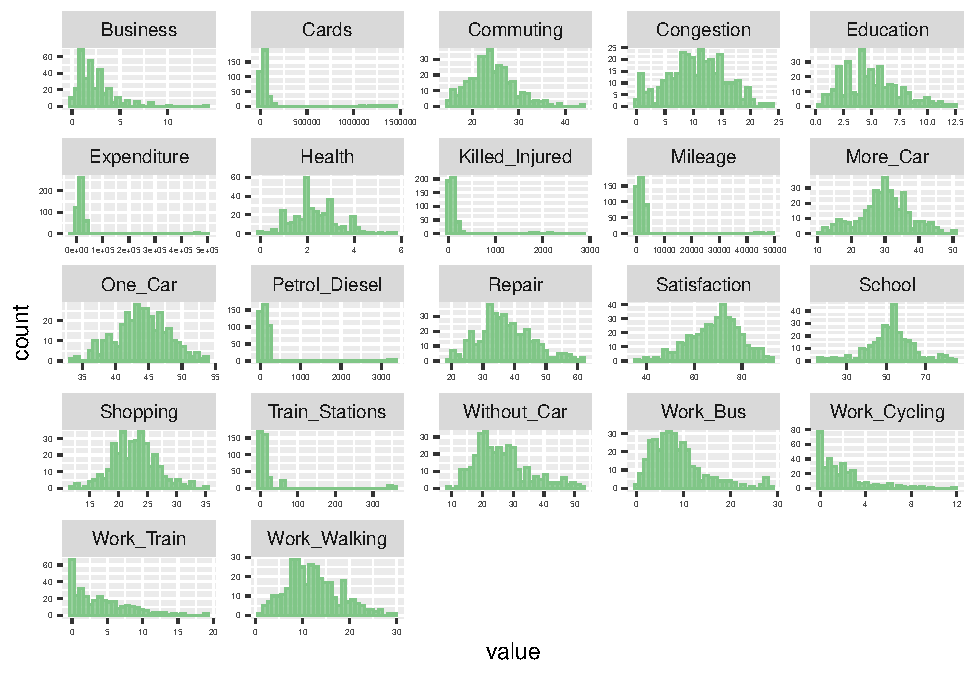
\includegraphics{RMD-Group-28_files/figure-latex/unnamed-chunk-3-1} 

}

\caption{\label{fig:his} Histogram plot of variables}\label{fig:unnamed-chunk-3}
\end{figure}

\begin{figure}[H]

{\centering 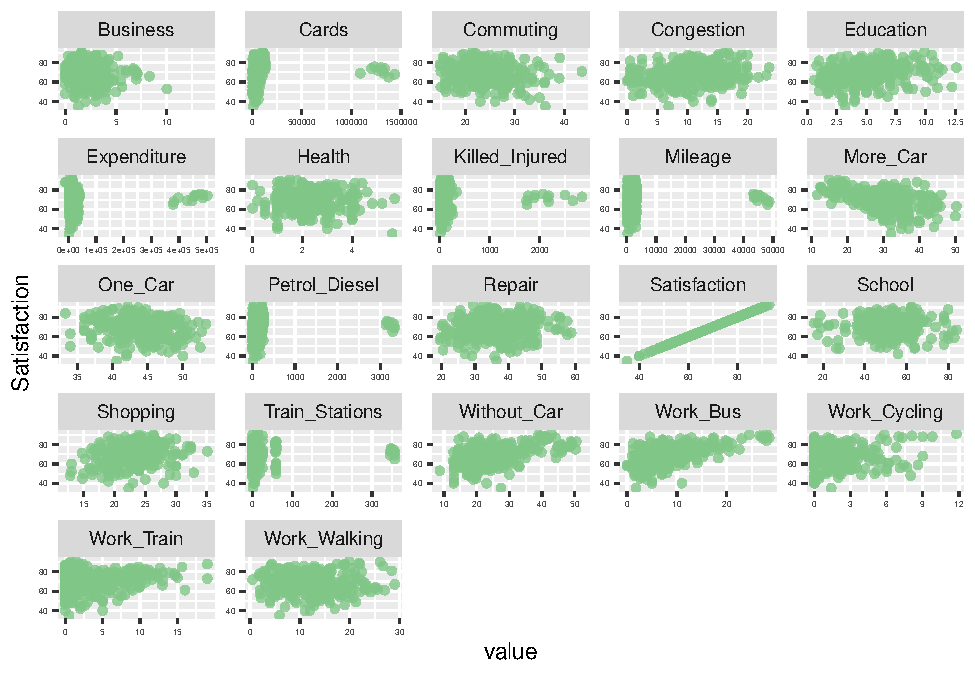
\includegraphics{RMD-Group-28_files/figure-latex/unnamed-chunk-4-1} 

}

\caption{\label{fig:scatter} Scatter plot of dependent variabls vs response variable}\label{fig:unnamed-chunk-4}
\end{figure}

\begin{figure}[H]

{\centering 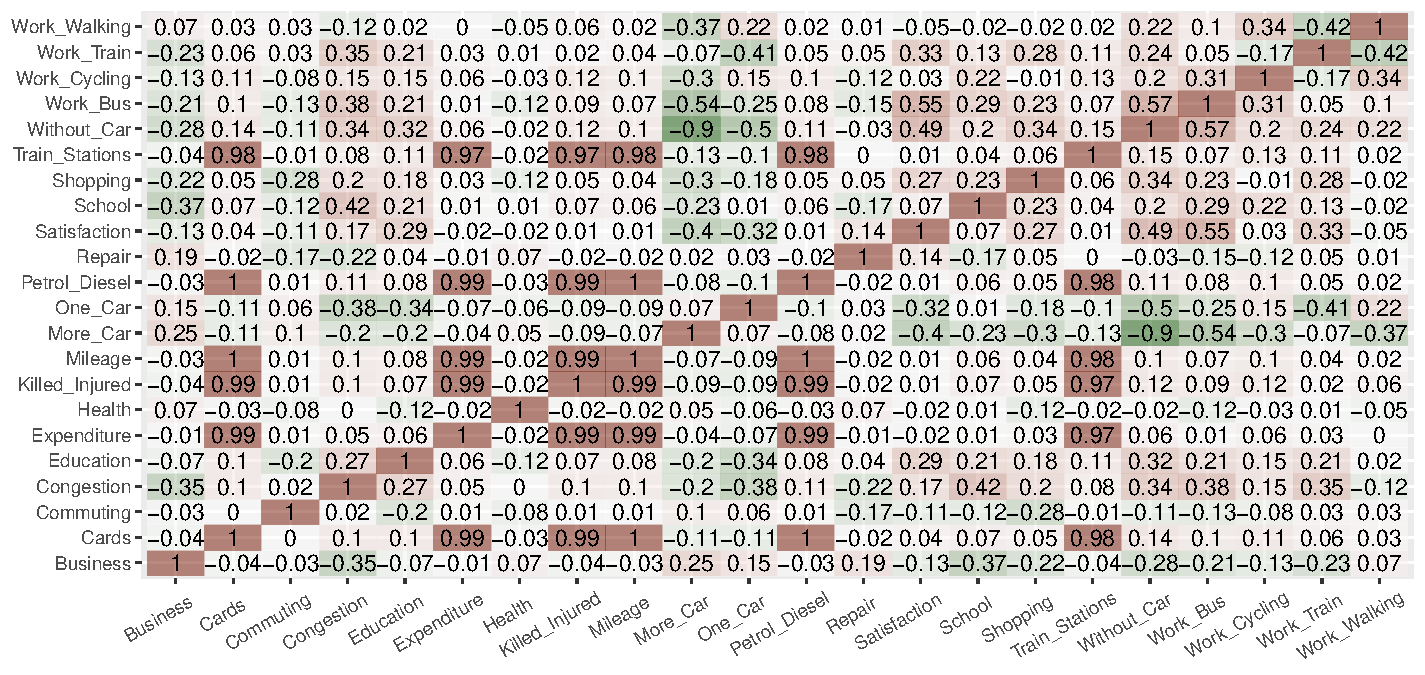
\includegraphics{RMD-Group-28_files/figure-latex/unnamed-chunk-5-1} 

}

\caption{\label{fig:cor} Correlation plot of variabls}\label{fig:unnamed-chunk-5}
\end{figure}

Through the correlation plot (Fig. \ref{fig:cor}), there is a strong
linear relationship between ``Petrol\_Diesel'' ``Train\_Stations'',
``Mileage'', ``Expenditure'', ``Killed\_Injured'' and ``Cards''. Then we
analyse the regression diagnosis results (Fig. \ref{fig:dia}) of model1
with all variables.

\begin{Shaded}
\begin{Highlighting}[]
\DocumentationTok{\#\#\#\# linear regression \#\#\#\#}
\CommentTok{\# full model}
\NormalTok{fit }\OtherTok{\textless{}{-}} \FunctionTok{lm}\NormalTok{(Satisfaction }\SpecialCharTok{\textasciitilde{}}\NormalTok{ ., }\AttributeTok{data =} \FunctionTok{na.omit}\NormalTok{(Data[, }\SpecialCharTok{{-}}\DecValTok{1}\NormalTok{]))}
\end{Highlighting}
\end{Shaded}

Plot the Fitted values against Residuals and Q-Q plot to assess our
assumptions.

\begin{figure}[H]

{\centering 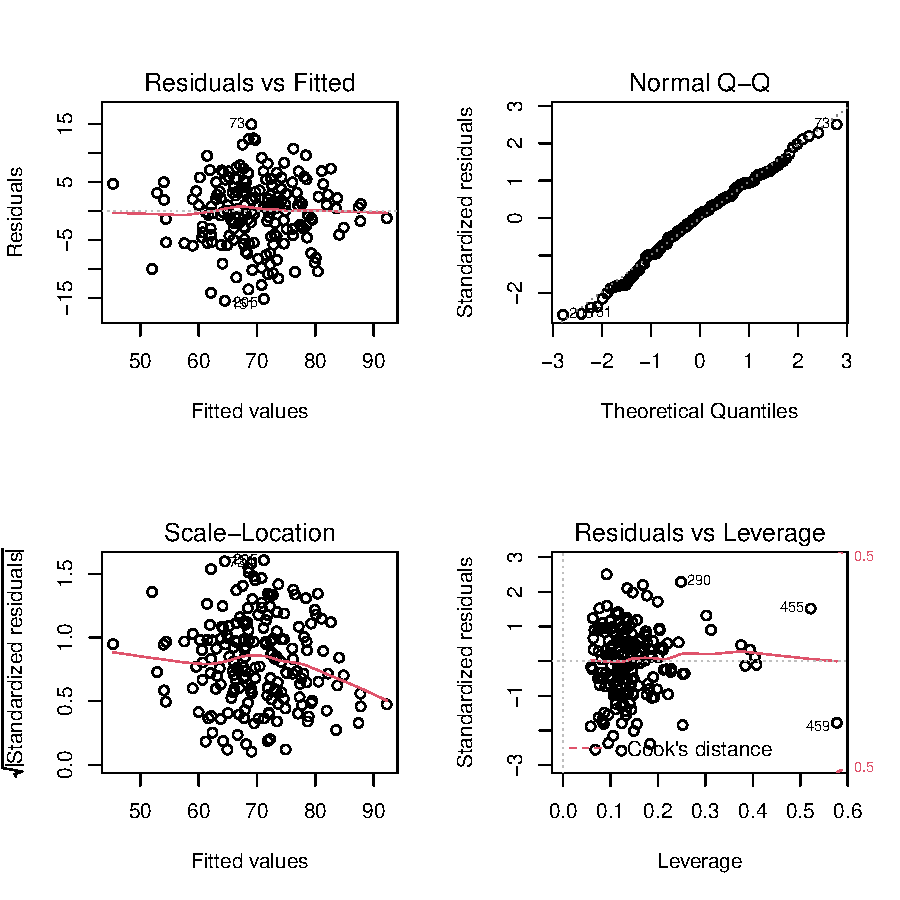
\includegraphics{RMD-Group-28_files/figure-latex/unnamed-chunk-7-1} 

}

\caption{\label{fig:dia} Regression diagnosis results}\label{fig:unnamed-chunk-7}
\end{figure}

\begin{itemize}
\item
  Residuals vs Fitted plot (left top) shows that there is no systematic
  correlation between the residual value and the fitting value.
\item
  Normal Q-Q plot (right top) shows the points on the graph fall on a
  straight line with an angle of 45 degrees, which indicates the
  assumption of normality is not violated.
\item
  Scale-location plot (left bottom) displays the points around the
  horizontal line are randomly distributed. The invariant variance
  assumption is satisfied.
\item
  Residuals vs leverage (right bottom) figures out special observations.
  The strong influence points do not deviate from the regression
  estimation seriously.
\item
  According to the correlation plot and VIF, there is obvious
  multicollinearity among variables.
\end{itemize}

\hypertarget{sec:FDA}{%
\section{Formal Data Analysis}\label{sec:FDA}}

Linear regression model, a model for examining and discovering relations
between the response variable and explanatory variable(s), is applied in
this project. The Satisfaction is the response variable, the DateCode is
the control variable and others are independent variables. A linear
regression model is applied as:
\[y=\beta_0+\beta_1x_1+\dots+\beta_px_p+\varepsilon \] where y is the
response variable, \(x_1\) to \(x_p\) is the number of columns selected
from 1 to p, \(\beta_0\) is the intercept of data, \(\beta_1\) to
\(\beta_p\) is the coefficients of corresponding columns of X from 1 to
p.~The \(\varepsilon\) is the error terms of the estimations.

\begin{Shaded}
\begin{Highlighting}[]
\CommentTok{\#library(MASS)}
\FunctionTok{library}\NormalTok{(MASS)}
\FunctionTok{stepAIC}\NormalTok{(fit, }\AttributeTok{na.rm =} \ConstantTok{TRUE}\NormalTok{)}

\CommentTok{\# 3 4 5 8 24}
\CommentTok{\# cards, killed\_injured, expenditure, petrol\_diesel, mileage are highly correlated.}
\CommentTok{\# model 2 without}
\FunctionTok{names}\NormalTok{(Data)[}\FunctionTok{c}\NormalTok{(}\DecValTok{3}\NormalTok{, }\DecValTok{4}\NormalTok{, }\DecValTok{5}\NormalTok{, }\DecValTok{8}\NormalTok{, }\DecValTok{24}\NormalTok{)]}

\NormalTok{fit2 }\OtherTok{\textless{}{-}} \FunctionTok{lm}\NormalTok{(Satisfaction }\SpecialCharTok{\textasciitilde{}}\NormalTok{ DateCode }\SpecialCharTok{+}\NormalTok{ Cards }\SpecialCharTok{+}\NormalTok{ Repair }\SpecialCharTok{+}\NormalTok{ Work\_Bus }\SpecialCharTok{+} 
\NormalTok{             School }\SpecialCharTok{+}\NormalTok{ Health }\SpecialCharTok{+}\NormalTok{ Work\_Train }\SpecialCharTok{+}\NormalTok{ Train\_Stations }\SpecialCharTok{+}\NormalTok{ Without\_Car }\SpecialCharTok{+} 
\NormalTok{             Petrol\_Diesel, }\AttributeTok{data =} \FunctionTok{na.omit}\NormalTok{(Data[, }\SpecialCharTok{{-}}\DecValTok{1}\NormalTok{]))}
\FunctionTok{summary}\NormalTok{(fit2)}

\DocumentationTok{\#\#\#\# Model selection \#\#\#\#}

\FunctionTok{glance}\NormalTok{(fit)}
\FunctionTok{glance}\NormalTok{(fit2)}
\end{Highlighting}
\end{Shaded}

A total of four regressions were performed. First, all the independent
variables were regressed, and then the highly correlated factors were
sequentially removed, and finally, four models were obtained. The
variables with high correlation are removed by stepwise regression. Step
AIC method is applied as a criterion for model selection. The model 2 is
the best choice. Stepwise regression technique is applied to model
selection. The selected model is as Table. \ref{tab:model2}. Control
variable ``DateCode'' isn't displayed.

\begin{table}

\caption{\label{tab:unnamed-chunk-9}Model2, selected by Stepwise regression\label{tab:model2}}
\centering
\begin{tabular}[t]{l|r|r|r|r}
\hline
term & estimate & std.error & statistic & p.value\\
\hline
(Intercept) & 52.9775625 & 3.9466689 & 13.4233613 & 0.0000000\\
\hline
Cards & 0.0001289 & 0.0000352 & 3.6559946 & 0.0003356\\
\hline
Repair & 0.2494980 & 0.0665578 & 3.7485909 & 0.0002391\\
\hline
Work\_Bus & 0.7333901 & 0.1074918 & 6.8227543 & 0.0000000\\
\hline
School & -0.1207559 & 0.0485715 & -2.4861470 & 0.0138198\\
\hline
Health & 0.2824925 & 0.5313962 & 0.5316043 & 0.5956519\\
\hline
Work\_Train & 0.7066629 & 0.1314720 & 5.3750078 & 0.0000002\\
\hline
Train\_Stations & -0.1537078 & 0.0468778 & -3.2789066 & 0.0012497\\
\hline
Without\_Car & 0.1676106 & 0.0740901 & 2.2622533 & 0.0248705\\
\hline
Petrol\_Diesel & -0.0367942 & 0.0146720 & -2.5077725 & 0.0130293\\
\hline
\end{tabular}
\end{table}

Model diagnosis are carried out to check model assumptions. Stepwise
regression is applied to select variables with AIC as the criterion.
Compare the selected model with full model on \(adj\) \(R^2\), AIC and
BIC. Model2 has higher \(adj\) \(R^2\) and smaller AIC and BIC compared
with the model1 as Table. \ref{tab:com}.

\begin{table}

\caption{\label{tab:unnamed-chunk-10}Comparison of model1 with model2 on adj R2, AIC and BIC\label{tab:com}}
\centering
\begin{tabular}[t]{l|r|r|r}
\hline
model & adj.r.squared & AIC & BIC\\
\hline
model 1 & 0.5478475 & 1271.288 & 1365.604\\
\hline
model 2 & 0.4998739 & 1274.555 & 1310.330\\
\hline
\end{tabular}
\end{table}

Therefore the model2 is better.

To obtain robust results, using Bootstrap to select significant
variables at 95\% level and obtain its confidence interval of parameter
estimation and their observations.This process should be repeated 1000
times.

\begin{Shaded}
\begin{Highlighting}[]
\NormalTok{boot\_models }\OtherTok{\textless{}{-}} \FunctionTok{bootstraps}\NormalTok{(Data[, }\SpecialCharTok{{-}}\DecValTok{1}\NormalTok{], }\AttributeTok{times =} \DecValTok{1000}\NormalTok{, }\AttributeTok{apparent =} \ConstantTok{TRUE}\NormalTok{) }\SpecialCharTok{\%\textgreater{}\%}
  \FunctionTok{mutate}\NormalTok{(}
    \AttributeTok{model =} \FunctionTok{map}\NormalTok{(splits, }\SpecialCharTok{\textasciitilde{}} \FunctionTok{lm}\NormalTok{(Satisfaction }\SpecialCharTok{\textasciitilde{}}\NormalTok{ DateCode }\SpecialCharTok{+}\NormalTok{ Cards }\SpecialCharTok{+}\NormalTok{ Repair }\SpecialCharTok{+}\NormalTok{ Work\_Bus }\SpecialCharTok{+} 
\NormalTok{                               School }\SpecialCharTok{+}\NormalTok{ Health }\SpecialCharTok{+}\NormalTok{ Work\_Train }\SpecialCharTok{+}\NormalTok{ Train\_Stations }\SpecialCharTok{+}\NormalTok{ Without\_Car }\SpecialCharTok{+} 
\NormalTok{                               Petrol\_Diesel, }\AttributeTok{data =}\NormalTok{ .)),}
    \AttributeTok{coef\_info =} \FunctionTok{map}\NormalTok{(model, tidy)}
\NormalTok{  )}

\NormalTok{boot\_coefs }\OtherTok{\textless{}{-}}\NormalTok{ boot\_models }\SpecialCharTok{\%\textgreater{}\%}
  \FunctionTok{unnest}\NormalTok{(coef\_info)}

\NormalTok{ci }\OtherTok{\textless{}{-}} \FunctionTok{int\_pctl}\NormalTok{(boot\_models, coef\_info)}
\CommentTok{\# significant at 0.05}
\NormalTok{sig }\OtherTok{\textless{}{-}}\NormalTok{ ci[}\FunctionTok{sign}\NormalTok{(ci[, }\DecValTok{2}\NormalTok{]) }\SpecialCharTok{==} \FunctionTok{sign}\NormalTok{(ci[, }\DecValTok{4}\NormalTok{]), ] }\SpecialCharTok{\%\textgreater{}\%} \FunctionTok{pull}\NormalTok{(term)}

\NormalTok{boot\_coefs }\OtherTok{\textless{}{-}}\NormalTok{  boot\_coefs }\SpecialCharTok{\%\textgreater{}\%}
  \FunctionTok{mutate}\NormalTok{(}\AttributeTok{sig =} \FunctionTok{ifelse}\NormalTok{(term }\SpecialCharTok{\%in\%}\NormalTok{ sig, }\StringTok{"TRUE"}\NormalTok{, }\StringTok{"FALSE"}\NormalTok{)) }\SpecialCharTok{\%\textgreater{}\%}
  \FunctionTok{filter}\NormalTok{(term }\SpecialCharTok{\%in\%} \FunctionTok{c}\NormalTok{(}\StringTok{"Cards"}\NormalTok{, }\StringTok{"Health"}\NormalTok{, }\StringTok{"Petrol\_Diesel"}\NormalTok{,}\StringTok{"Repair"}\NormalTok{, }\StringTok{"School"}\NormalTok{, }\StringTok{"Train\_Stations"}\NormalTok{, }\StringTok{"Without\_Car"}\NormalTok{, }\StringTok{"Work\_Bus"}\NormalTok{, }\StringTok{"Work\_Train"}\NormalTok{))}

\NormalTok{boot\_coefs2 }\OtherTok{\textless{}{-}}\NormalTok{ boot\_coefs }\SpecialCharTok{\%\textgreater{}\%}
  \FunctionTok{group\_by}\NormalTok{(term) }\SpecialCharTok{\%\textgreater{}\%}
  \FunctionTok{summarise}\NormalTok{(}\AttributeTok{est =} \FunctionTok{median}\NormalTok{(estimate), }\AttributeTok{lower =} \FunctionTok{quantile}\NormalTok{(estimate, }\FloatTok{0.025}\NormalTok{), }\AttributeTok{upper =} \FunctionTok{quantile}\NormalTok{(estimate, }\FloatTok{0.975}\NormalTok{))}

\NormalTok{boot\_coefs }\SpecialCharTok{\%\textgreater{}\%}
  \FunctionTok{ggplot}\NormalTok{() }\SpecialCharTok{+}
  \FunctionTok{geom\_density}\NormalTok{(}\FunctionTok{aes}\NormalTok{(estimate, }\AttributeTok{fill =}\NormalTok{ sig), }\AttributeTok{alpha =} \FloatTok{0.7}\NormalTok{,  }\AttributeTok{color =} \StringTok{"white"}\NormalTok{) }\SpecialCharTok{+}
  \FunctionTok{geom\_vline}\NormalTok{(}\AttributeTok{data =}\NormalTok{ boot\_coefs2, }\AttributeTok{mapping =} \FunctionTok{aes}\NormalTok{(}\AttributeTok{xintercept =}\NormalTok{ est))}\SpecialCharTok{+}
  \FunctionTok{geom\_vline}\NormalTok{(}\AttributeTok{data =}\NormalTok{ boot\_coefs2, }\AttributeTok{mapping =} \FunctionTok{aes}\NormalTok{(}\AttributeTok{xintercept =}\NormalTok{ lower), }\AttributeTok{color=}\StringTok{"Red"}\NormalTok{, }\AttributeTok{lty =} \DecValTok{2}\NormalTok{)}\SpecialCharTok{+}
  \FunctionTok{geom\_vline}\NormalTok{(}\AttributeTok{data =}\NormalTok{ boot\_coefs2, }\AttributeTok{mapping =} \FunctionTok{aes}\NormalTok{(}\AttributeTok{xintercept =}\NormalTok{ upper), }\AttributeTok{color=}\StringTok{"Red"}\NormalTok{, }\AttributeTok{lty =} \DecValTok{2}\NormalTok{)}\SpecialCharTok{+}
  \FunctionTok{geom\_vline}\NormalTok{(}\AttributeTok{data =}\NormalTok{ boot\_coefs2, }\AttributeTok{mapping =} \FunctionTok{aes}\NormalTok{(}\AttributeTok{xintercept =} \DecValTok{0}\NormalTok{), }\AttributeTok{color=}\StringTok{"Blue"}\NormalTok{, }\AttributeTok{lty =} \DecValTok{2}\NormalTok{)}\SpecialCharTok{+}
  \FunctionTok{facet\_wrap}\NormalTok{(}\SpecialCharTok{\textasciitilde{}}\NormalTok{term, }\AttributeTok{scales =} \StringTok{"free"}\NormalTok{)}\SpecialCharTok{+}
  \FunctionTok{theme}\NormalTok{(}\AttributeTok{axis.text.x=} \FunctionTok{element\_text}\NormalTok{(}\AttributeTok{size =} \DecValTok{6}\NormalTok{),}
        \AttributeTok{axis.text.y=} \FunctionTok{element\_text}\NormalTok{(}\AttributeTok{size =} \DecValTok{6}\NormalTok{))}
\end{Highlighting}
\end{Shaded}

\begin{figure}[H]

{\centering 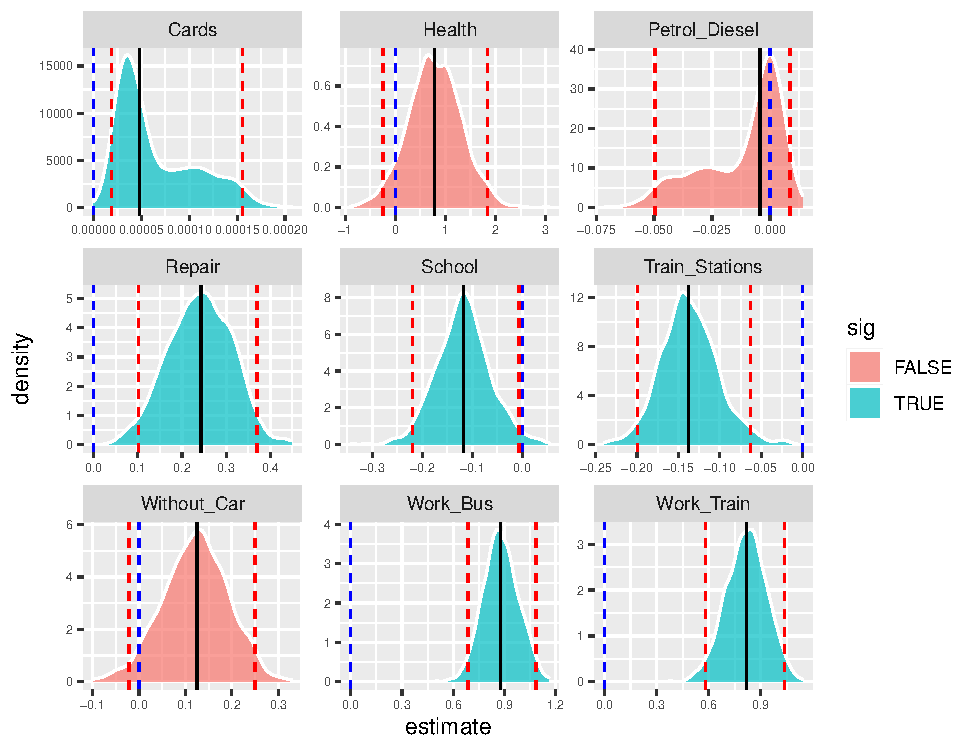
\includegraphics[width=0.8\linewidth]{RMD-Group-28_files/figure-latex/unnamed-chunk-11-1} 

}

\caption{Density plots of parameters via bootstrap\label{fig:boot}}\label{fig:unnamed-chunk-11}
\end{figure}

The density plots (Fig. \ref{fig:boot}) of parameters are displayed. The
variables with orange are not significant while the variables with blue
are significant at the \(\alpha=0.05\). The blue dashed lines are zero
and the orange dashed lines are 95\% CI of parameters. The black lines
are estimations of parameters.

\hypertarget{sec:Conc}{%
\section{Conclusions}\label{sec:Conc}}

\begin{itemize}
\item
  The variables Cards (Number of concessionary cards issued to all
  adults), Repair (The Percentage of Roads Needing Repairs), Work\_Bus
  (Bus Journeys To Work) and Work\_Train (Train Journeys To Work) have
  positive influence on satisfaction with public transport. The School
  (Child Journeys To School By Walking/Cycling) and Train\_Stations
  (Number of Train Stations) have negative relationship with
  satisfaction with public transport.
\item
  The reason that more roads needing repairs and less train stations
  come with higher satisfaction needs to be further explored.
\end{itemize}

\hypertarget{sec:Ref}{%
\section{References}\label{sec:Ref}}

\begin{itemize}
\item
  Jim Hester and Hadley Wickham, (2020). \emph{fs: Cross-Platform File
  System Operations Based on `libuv'.} R package version 1.5.0
\item
  Kuhn et al., (2020). \emph{Tidymodels: a collection of packages for
  modeling and machine learning using tidyverse principles}.
\item
  Wickham et al., (2019). \emph{Welcome to the tidyverse. Journal of
  Open Source Software}, e, 4(43), 1686
\end{itemize}

\end{document}
